\section{Method} \label{sec:method}
	The optimization of power regulation while minimizing loads, requires a model that can describe the power output and the loads of a wind farm. This section describes how this in implemented \newline
	An overview of the optimization procedure used is illustrated in Figure \ref{fig:optim}.
	The power output of a wind farm as well as the wake propagation in this wind farm are calculated using the FLORIS model \cite{FLORIS} (Section \ref{sec:floris}). Given a certain inflow profile the program FAST calculates the out of plane bending moments on a turbine. With the program MLife these bending moments are converted to a Damage Equivalent Load (DEL), which is a measure for the lifespan of a wind turbine \cite{MLife}. Both FAST and MLife are covered in Section \ref{sec:fast}. These DELs are pre-calculated for different situations, which are specified by four parameters, and stored in a look-up-table (LUT) so it can be quickly retrieved during optimization (Section \ref{sec:lut}). The optimization algorithm uses a cost function that combines the DEL and power data to find the optimal wind turbine configuration that has minimal loads while tracking a predefined reference power (Section \ref{sec:optimization}).

	\begin{figure}
		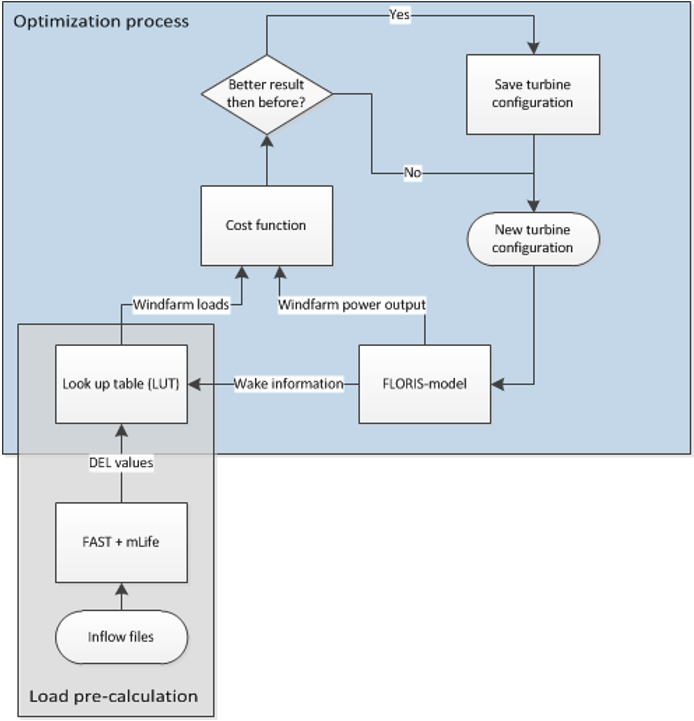
\includegraphics[width=\linewidth]{./Figures/OptimizationProcess.png}
		\caption{Overview of the optimization procedure.}
		\label{fig:optim}
	\end{figure}


%\noindent

\subsection{FLORIS} The FLORIS, or FLOw Redirection and Induction in Steady state, model is used for the generation of wake propagation and power output data of windfarms as a function of the yaw misalignment and the axial induction\cite{Gebraad2016}.
FLORIS is a relative accurate model\cite{Dijk2016} with a relatively low computation time, since it is a parametric model fitted to high-fidelity data from a computational fluid dynamics simulation. 

\subsubsection{Wake modelling}
\label{wakemodel}
%As can be seen in Figure \ref{fig:wake}, 
FLORIS generates a wake model which divides the wake into three different zones as shown in Figure\ref{fig:wake}. These zones are as the near wake, the far wake, and the mixing zone, and are denoted by $q$. Each zone has its own diameter and wind speed, which are calculated by FLORIS using Equations(\ref{eq:Dw} to \ref{eq:c}). 


\begin{figure}
  	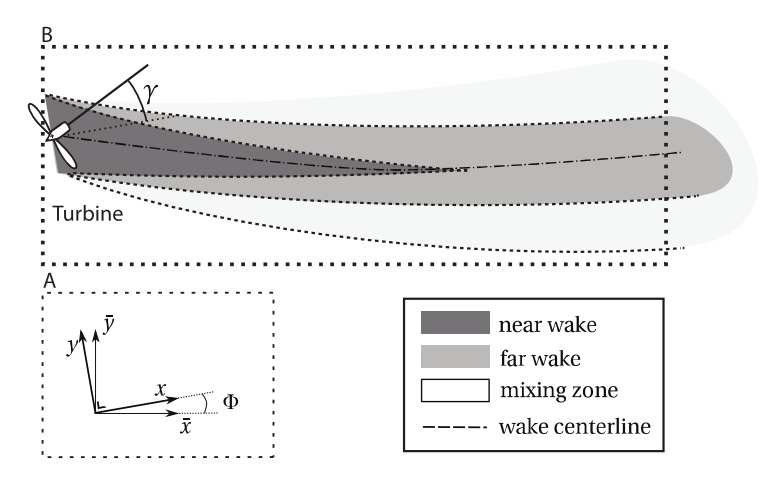
\includegraphics[width=\linewidth]{./Figures/WakeFLORIS.png}
  	\caption{Simplified top view representation of a wake of a turbine by FLORIS.\cite{Gebraad2016}   }
	\label{fig:wake}
\end{figure}

The size of the wake diameter is calculated using Eq \ref{eq:Dw}. let the $D_i$ denote the rotor diameter of the $i${\textsuperscript{th}} turbine, $k_e$ a coefficient that describes expansion of the zones, and $m_{e,q}$, the expansion factor as used by Gebraad\cite{Gebraad2016}. The size of the wake diameter $D_{w,q,i}$ increases proportionally to the downwind distance ($x$). 
\begin{equation}
\label{eq:Dw}
D_{w,i,q}(x) = max({D_i + 2k_em_{e,q}([x - X_i],0} )
\end{equation}
The wake velocity depends on the downwind distance $(x)$ as well. As shown in Eq \ref{eq:Uw}, is the wake velocity an argument of the wake decay coefficient $c(x,y)$ (<--). This wake decay coefficient is multiplied by the axial induction factor and subtracted from the free stream velocity $U_i$. The axial induction factor is a value for the decrease in wind velocity behind a turbine relative to its own rotor speed. The wake decay coefficient describes the decay of velocity for each wake zone and is defined in \ref{eq:c}. The model parameter $M_{U,q}$, which depends on the wake zone and the yaw angle, is calculated by Gebraad.\cite{Gebraad2016}   

\begin{equation}
\label{eq:Uw}
U_{w,i}(x,y) = U_i\left( {1-2a_ic_i(x,y)} \right)
\end{equation} 

\begin{equation}
\label{eq:c}
c_{i,q}(x) = \left[ \frac{D_i}{D_i + 2k_em_{U,q}(\gamma_i)[x - X_i]} \right]^2
\end{equation}




%\noindent

\subsection{FAST \& MLife} FAST is a programming tool for the simulation of dynamic (load) responses of wind turbines (by NREL) \cite{Jonkman2005}. It computes the bending moment of a blade given (defineerbare/...) input data. Since the bending moment of a blade does not give direct information about the effect on the life-cycle time of a turbine, the program MLife is used to convert the bending moment to damage equivalent loads (DELs). (these DELs are better why??)


\begin{figure}
  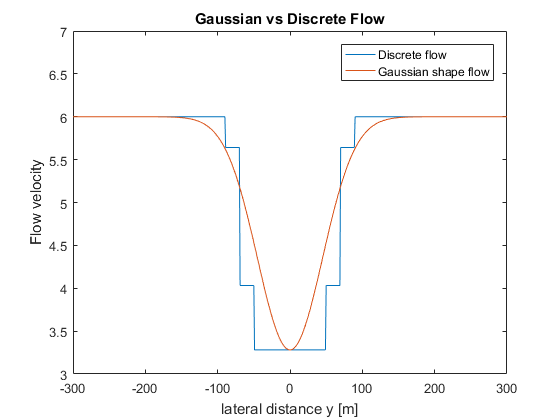
\includegraphics[width=\linewidth]{./Figures/PlotGausDiscWakeDWake180U6yaw0.png} %Plot with Gauss vs Discr flow, Dwake = 180, u_mean = 6, yaw = 0
  \caption{Discrete wake versus Gaussian wake} %for Dwake = 180 m, U = 6 m/s, and yaw = 0
  \label{fig:disgaus}
\end{figure}

%\noindent

\subsubsection{Flow field}
FAST uses external input files as input for the simulation data. This paper mostly used the flow field as input towards FAST. 
more intro:... making it more representative for real life, by implementing both a more acurate flow distribution as natural fenomena.

\paragraph{Gaussian wake}
FLORIS describes a discrete flow field of a wake, with three zones. The flow field of the wake in FLORIS is calculated with equations (\ref{eq:Dw} to \ref{eq:c}). The wake is divided into three zones as described in section \ref{wakemodel}. A real wake, however, does not have these discrete zones. To create a more fluent transition between the different wake-zones a Gaussian distribution of the flow field is chosen \cite{Bastankhah2016}. The wake shape difference can be seen in Figure \ref{fig:disgaus}.  The Gaussian distribution is calculated as follows: 

\begin{equation}
\label{eq:gaus}
G(y, z) = A [e^{-(\frac{y^2}{2\sigma_y} + \frac{z^2}{2\sigma_z})}]
\end{equation}
The amplitude of the Gaussian, $A$, is set to be equal to the velocity loss of the inner wake zone, $U_{w,1}$, as FLORIS models it(!!verwoording mag anders). $\sigma_y$ and $\sigma_z$ reflect the Gaussian standard deviation in horizontal and vertical direction, respectively. These standard deviations are related to the outer wake zone $D_{w,i,q=3}$ following Equation \ref{eq:sigm},
\begin{equation}
\label{eq:sigm}
\sigma_y,\sigma_z = D_{w,i,q=3}/n 
\end{equation}
\\
Where fit parameter $n$ can be modified to change the width of the Gaussian. Consequently, making it possible to fit the Gaussian to the wake zones of FLORIS. (Figure \ref{fig:disgaus})
(clearly note the relation between the gausian and the wakes from FLORIS)

\paragraph{Wind shear} \label{sec:windshear}
An other aspect added to inprove the the wind ... is wind shear, this is an natural phenomanen. opstructions and earth surface roughnes cause the wind to slow down closer to earth. This causes a significant diferance in windspeed over the hight ranges of the turbine\cite{Firtin2011}.  The velocity distribution is calculated as follows: 
\begin{equation}
\label{eq:shear}
v = v_{ref} \left[\frac{h}{h_{ref}}\right]^\alpha
\end{equation}
where $v$ and $v_{ref}$ are the velocity at heights $h$, and $h_{ref}$  respectively. Value $\alpha$ is the wind shear coefficient which depends on different factors. The coefficient $\alpha$  reflects terrain type, and is for this paper fixed at value 0.1 representing a surface close to ocean and smooth ground \cite{Firtin2011}. The difference between a flow field with and without wind shear can be seen in Figure \ref{fig:windshear}

\begin{figure}
	\centering
	\begin{subfigure}[b]{0.50\textwidth}
		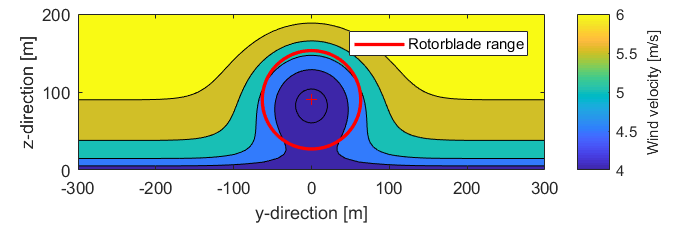
\includegraphics[width=\linewidth]{./Figures/PlotwithshearU6D220.png} %Plot with windshear u_mean = 6
		\caption{Flow field with wind shear.}
		\label{fig:windsh}
	\end{subfigure}
	
	\begin{subfigure}[b]{0.50\textwidth}
		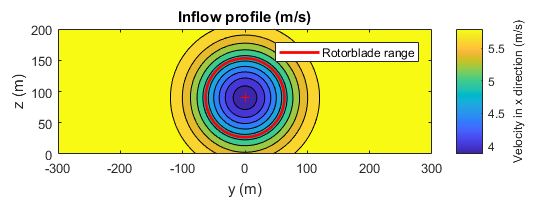
\includegraphics[width=\linewidth]{./Figures/PlotwithoutshearU6D220.png} %Plot without windshear u_mean = 6
		\caption{Flow field without wind shear}
		\label{fig:nowindsh}
	\end{subfigure}
	
	\caption[Two Gaussian flow fields]{Gaussian wind fields with a free stream velocity of 6 $m/s$ at a height of 90 $m$. The outer diameter of de wake is 220 $m$ and the diameter of the rotor blades is 126.4 $m$.}
	\label{fig:windshear}
\end{figure}




\begin{table}[h]
	%\renewcommand{\arraystretch}{1.3} 
	\caption{Overview of the minimum value, maximum value, and step size of the parameters, diameter of outer wake zone (Dwake), free stream wind speed (U), yaw of the turbine (yaw), and the center to center distance between the center of the turbine and the center of the wake (y wake).}
	\centering
	\label{tab:pars}
	\begin{tabular}{lccc}
		\hline
	 	& Minimum & Maximum & Step-size \\ 
		\hline
		Dwake & 180 & 330 & 25 \\
		U & 6 & 8 & 2 \\
		yaw & -30 & 30 & $^*$ \\
		y wake & -250 & 250 & 10 \\
		\hline
	\end{tabular}
$^*$Input values for yaw are [-30, -10, -5, 0, 5, 10, 30].
\end{table}

%\noindent
\subsection{LUT} \label{sec:lut}
 To reduce computational time during optimization a look-up table (LUT) is created. The LUT is created using FAST and MLife, and it contains a a large number of DEL values for a wide variety of wind field conditions on a wind turbine.
These different conditions are described by the ranges of the parameters, which can be seen in Table \ref{tab:pars}. The parameters are wake characteristics which can be extracted from FLORIS. The parameters chosen for the LUT are:\begin{itemize}
	\item the free stream wind speed, U
	\item the outer diameter of the wake, Dwake
	\item the yaw of the turbine, yaw  
	\item the center to center distance between the turbine and the wake, y wake 
\end{itemize}   
 To save calculation time, the LUT parameters are discretized, given each parameter a certain step-size. This step-size is chosen such that interpolation will give a representative result. For each parameters step-sizes are selected, as shown in Table \ref{tab:pars}. With the use of the pre-calculated LUT, online optimization can be realized.



 This paper uses the wake diameter as a parameter to characterise the wakes. However, as stated before are the diameter of the wake, the downwind distance and the windspeed reduction behind the turbine(Udef) related by fitting equations. This means that the distance and the Udef could have been used as parameter just as well. The choice for the diameter comes since Floris searches for the best fit of the shape of a wake in the LUT data. And the diameter gives a more direct interpretation of the shape of the wake than the others do, subsequently meaning that the diameter comes more intuitively.

 
 

%\noindent
\subsection{Optimization} \label{sec:optimization}
To optimize for power reference tracking and load minimization, a game-theoretic approach was used.\cite{Marden2013} The optimization algorithm searches for the optimal yaw and axial induction settings of each individual turbine. These can influence the power and loads significantly, so both are combined in a cost function. \cite{Marden2013}\cite{Dijk2016} 

\subsubsection{Cost Function} \label{sec:costfunction}
The cost function depends on two variables: a normalized power and a normalized load variable. To achieve the optimal yaw and axial induction settings a mixed-objective cost function is defined as follows:

\begin{equation}
\begin{aligned}
J(P,DEL) = c*((P_{ref}-P(a_i,\gamma_i))/P_{bw})^2  + \\
(1-c)*DEL(a_i,\gamma_i)/DEL_{base}
\end{aligned}
 \label{eq:costf}
\end{equation}
Where $c$ is the tuning parameter for the optimization between power and loads and $P_{ref}$ is the desired power output of the wind farm. $P_{bw}$ and $DEL_{base}$ are the power and loads baselines respectively, to create normalized variables.
\newline
To execute the optimization, the cost function has to be minimized. To obtain power production close to the reference, the power part of the cost function is a quadratic difference. As a result values much larger than the reference are heavily penalized, whereas the power crosses $P_{bw}$ the emphasis shifts to the loads.

\subsubsection{Game Theory} \label{sec:gametheory}
The game-theoretic approach uses random perturbations for the yaw angles and the axial induction to optimize the cost function. When new values for yaw and axial induction settings give an improvement regarding the cost function, the settings are saved and the process will be repeated with the new settings. Because of the fact it uses random perturbations, the game theoretic approach is an adequate optimizer to find the global minimum of the cost function.\cite{Dijk2016}




